\documentclass{article}
\usepackage[utf8]{inputenc}
\usepackage[margin=1.2in]{geometry}
\usepackage{hyperref}

\usepackage{tikz}
\usetikzlibrary{positioning}

\usepackage{natbib}
\usepackage{graphicx}
\usepackage{amsmath}

\title{\vspace{-2 cm}Universidade Federal de Ouro Preto \\ BCC 325 - Inteligência Artificial \\ Busca em Espaço de Estados}
\author{Prof. Rodrigo Silva}
\date{}


\begin{document}

\maketitle

\section{Leitura}

\begin{itemize}
    \item Capítulo 3 do Livro\textit{ Artificial Intelligence: Foundations of Computational Agents,  2nd Edition} disponível em \textit{https://artint.info/}
\end{itemize}

\section{Questões}

\begin{enumerate}
    \item (Seção 3.1) O que significa busca no contexto dos métodos que iremos estudar?
    \item (Seção 3.2) Quais são as premissas de um problem de busca em espcaços de estados?
    \item (Seção 3.2) Quais são os componentes de um problema de busca em espacos de estados?
    \item (Seção 3.3) Qual a relação entre espaços de estados e grafos?
    \item (Seção 3.3.1) Quais os componente e os objetivos de um problema de busca em grafos?
    \item (Seção 3.4) Apresente o algoritmo genérico de busca?
    \item (Seção 3.5.1) Apresente um exemplo de execução do algoritmo de busca em profundidade. (Apresente o estado da fronteira a cada interação.)
    \item (Seção 3.5.2) Apresente um exemplo de execução do algoritmo de busca em largura.(Apresente o estado da fronteira a cada interação.)
\end{enumerate}



%\section{Projeto}

%\begin{enumerate}
%\item Nesta atividade você deve desenvolver um sistema agente/ambiente em que o agente explora um campo com obstáculos (ambiente). Dada um posição inicial e uma posição final, o agente deve encontrar o caminho de uma até a outra, desviando dos obstáculos, utilizando os seguinte algoritmos de busca:

%\begin{enumerate}
%    \item Busca em largura
%    \item Busca em profundidade
%    \item Algoritmo guloso
%    \item Menor custo primeiro
%    \item A*
%    \item Branch-and-bound
%\end{enumerate}

%\item  Preencha a seguinte tabela com experiência adquirida no projeto

%\begin{center}
%        \begin{tabular}{|l|c|c|c|}
%        \hline
%        Estratégia            & Seleção da fronteira & Caminho Encontrado & Custo em Espaço \\
%        \hline
%        Busca em Largura      &     &   &   \\
%        \hline
%        Busca em Profundidade &     & (g)  &   \\
%        \hline
%        Guloso                &     &   &   \\
%        \hline
%        Menor Caminho Primeiro& (b) &   &   \\
%        \hline
%        $A^*$                 &     &   &   \\
%        \hline
%        Branch and Bound      &     &   &   \\
%        \hline
%    \end{tabular}
%    \end{center}
    
%    \begin{enumerate}
%        \item Menor $h(n)$
%        \item Menor $c(S,n)$
%        \item Menor $h(n) + c(S,n)$
%        \item Primeiro caminho adicionado 
%        \item Último caminho adicionado 
%        \item Menor número de arcos
%        \item Indefinido
%        \item Menor custo
%        \item Linear 
%        \item Exponencial
%    \end{enumerate}
%\end{enumerate} 


   
% Na leitura recomendada você deve ter lido que agentes são entidades que interagem com um ambiente. Nesta atividade você deve implementar agentes que encontram o caminho de uma posição inicial até uma posição alvo desviando de objetos. 

% Visite o repositório \url{https://github.com/rcpsilva/BCC740\_ArtificialIntelligence}, que contem o código base para esta atividade e leia atentamente o README.

% O arquivo \textit{Room.py} contém a classe \texttt{Room} que implementa um \texttt{Environment} que representa uma sala com obstáculos. Atributos importantes desta classe são:

% \begin{itemize}
%     \item \texttt{room}: É uma matriz que contém 0 nas posições livres e 0 nas posições com obstáculos.
%     \item \texttt{initial\_positon}: Posição inicial do agente na sala.
%     \item \texttt{target}: Posição em que o agente deve chegar.
% \end{itemize}

% O método de classe \texttt{initial\_percepts()} retorna:

% \begin{itemize}
%     \item \texttt{current\_position}: com a posição inicial do agente.
%     \item \texttt{target}: com a posição em que o agente deve chegar.
%     \item \texttt{neighboors} com as posições vizinhas livres. 
% \end{itemize}

% O método de classe \texttt{signal(action)} retorna:

% \begin{itemize}
%     \item \texttt{current\_position}: com a posição atual do agente.
%     \item \texttt{target}: com a posição em que o agente deve chegar.(Obs: Esta opção está aqui para modelar a possibilidade de mudança de objetivo durante a execução.)
%     \item \texttt{neighboors} com as posições vizinhas livres. 
% \end{itemize}

% Uma \texttt{action} é, da lista de vizinhos livres, a posição para onde o agente quer se mover. 

% Veja o exemplo ilustrado na figura \ref{fig:room}.

% \begin{figure}[!ht]
%     \centering
%     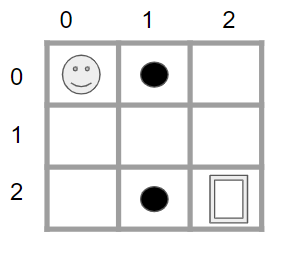
\includegraphics[width=0.4\textwidth]{room.PNG}
%     \caption{Ilustração da classe \texttt{Room}}
%     \label{fig:room}
% \end{figure}

% Para o exemplo mostrado na figura \ref{fig:room} teríamos:
%     \[
%         \texttt{room} = \begin{bmatrix}
%             0 & 1 & 0\\ 
%             0 & 0 & 0\\ 
%             0 & 1 & 0
%         \end{bmatrix}
%     \]
    
%     \[
%         \texttt{begin} = [0,0]
%     \]
    
%     \[
%         \texttt{target} = [2,2]
%     \]
    
%     \[
%         \texttt{current\_position} = [0,0]
%     \]
    
%     \[
%         \texttt{target} = [2,2]
%     \]
    
%     \[
%         \texttt{neighboors} = [[1,0],[1,1]]
%     \]

% o arquivo \textit{path\_finder\_agents.py} contém a implementação do \texttt{RandAgent}. Em cada posição, este agente escolhe um vizinho livre aleatoriamente para visitar. Ele para quando chega à posição alvo. Este agente pode ser usando como base para a implementação de outros agentes.

% Dadas estas informações, faça:

% \begin{enumerate}
%     \item Clone repositório \url{https://github.com/rcpsilva/BCC740\_ArtificialIntelligence}, leia atentamente o README e trabalhe a partir dele.
%     \item Execute o arquivo \textit{path\_finder\_simulation.py} para ver como o RandAgent se comporta.
%     \item No arquivo \textit{path\_finder\_agents.py}, implemente a classe \texttt{BFSAgent} que representa um agente que encontra a posição alvo fazendo uma busca em largura.
%     \item No arquivo \textit{path\_finder\_agents.py}, implemente a classe \texttt{DFSAgent} que representa um agente que encontra a posição alvo fazendo uma busca em profundidade.
%     \item No arquivo \textit{path\_finder\_agents.py}, implemente a classe \texttt{GreedyAgent} que representa um agente que encontra a posição alvo utilizando o algoritmo guloso.
%     \item No arquivo \textit{path\_finder\_agents.py}, implemente a classe \texttt{AStarAgent} que representa um agente que encontra a posição alvo utilizando o algoritmo A$^*$.
% \end{enumerate}

% Observações:
% \begin{itemize}
%     \item Todos os agentes implementados devem fazer poda de ciclos e poda de múltiplos caminhos.
%     \item Os agentes devem implementar a interface \texttt{Agent} definida no arquivo \textit{definitions.py}. 
%     \item Métodos auxiliares podem ser implementados para os agentes.
%     \item A classe $Room$ não deve ser modificada.
%     \item Os agentes implementados devem ser testados como indicado no arquivo \textit{path\_finder\_simulation.py}
% \end{itemize}
    

% %\bibliographystyle{plain}
% %\bibliography{references}
\end{document}

